\documentclass[11pt,a4paper]{report}
\usepackage[utf8]{inputenc}
\usepackage[french]{babel}
\usepackage[T1]{fontenc}
\usepackage{amsmath}
\usepackage{amsfonts}
\usepackage{amssymb}
\usepackage{graphicx}
\usepackage{makeidx}   
\usepackage{float}
\begin{document}
\begin{titlepage}
\newcommand{\HRule}{\rule{\linewidth}{0.5mm}}
\center
\textsc{\LARGE
Ecole Nationale Superieure Polytechnique de Maroua
} \\[1cm]
\textsc{\Large
Departement d'Informatique et Telecommunications
} \\[1cm]
\textsc{\large
\underline{UE} : Cryptographie avancee \\ \underline{CODE} : SEC519
} \\[1cm]
\HRule \\[0.4cm]
{ \huge \bfseries Rapport des Travaux Diriges 1  \\[0.15cm]}
\HRule \\[1.5cm]
KOUAM CHEKAM LEOPOLD JUNIOR \\
18A0265P \\[1cm]
MOGO KAMDEM ROOSEVELT\\
18A0308P \\[1cm]

TIL LA DJIBRIL SAMUEL\\
 
\today \\ [1cm]
\end{titlepage}
\newpage
\tableofcontents

\chapter*{INTRODUCTION}
\addcontentsline {toc}{chapter}{INTRODUCTION}
L'idée du gestionnaire de mot de passe vient du faite que nous devrions utiliser des mots de passe uniques et forts pour tous nos sites Web, nos comptes et nos applications.Cependant, il peut être difficile de créer des mots de passe différents, notamment si nous devions de respecter les normes de cybercriminalité en matière de complexité. Et garder un suivi de tous ces mots de passe peut suffire à nous donner des vertiges. Pour faciliter les choses, nous choisissons souvent des mots de passe simples, comme le nom de notre chien ou de notre enfant, ou nous réutilisons les mêmes mots de passe pour différents comptes. Cette façon de faire nous rend vulnérables face à des crimes comme le vol d'identité. Un pirate peut s’emparer de renseignements comme votre numéro de carte de crédit, votre adresse ou votre numéro d'assurance sociale pour contracter des emprunts, ouvrir des comptes de carte de crédit ou procéder à des achats. Nous n’avez donc pas le choix d’utiliser des mots de passe forts. C’est la raison pour laquelle il vous faut un gestionnaire de mots de passe. Tout au long de ce rapport nous vous présenterons notre solution de gestionnaire de mot de passe developpé que nous avons appélé \textbf{Safeprivacing.
}

\chapter{ÉTUDE DE L'EXISTANT}

Un gestionnaire de mots de passe peut vous aider à gérer de manière transparente toutes les données de connexion de vos appareils. Ces outils sont également pratiques pour remplir automatiquement des formulaires et synchroniser vos données sur PC, Mac Windows, iPhone, iPad, les smartphones Android, etc. Tous les gestionnaires de mots de passe présents dans notre sélection des meilleurs gèrent l'authentification matérielle avec une clé de sécurité YubiKey. Certains proposent des options payantes qui permettent de synchroniser des informations de connexion sur tous les appareils, d'accéder à un stockage en ligne sécurisé et de partager ses informations d'identification avec sa famille et amis de confiance.

\textbf{Bitwarden :} \\
meilleur gestionnaire en version gratuite, Open source, sécurisé et transparent
Bitwarden est en tête de la liste des meilleurs gestionnaires de mots de passe pour 2021 grâce à ses racines open-source et à sa version gratuite et illimitée. Ce logiciel de chiffrement allégé peut générer, stocker et remplir automatiquement vos mots de passe sur tous vos appareils et navigateurs populaires, y compris Brave et Tor.

Sa version gratuite est dépourvue de certaines des caractéristiques de nos autres choix, mais ses versions premium sont tout aussi riches en fonctionnalités. Tout comme ses concurrents les plus proches, l'abonnement premium de \textbf{Bitwarden} vous permet de partager des mots de passe, des identifiants, des adhésions et d'autres éléments avec des membres de votre famille et des amis de confiance, d'utiliser l'authentification multifactorielle via YubiKey et de bénéficier d'un gigaoctet de stockage chiffré. Bien qu'elle ait moins de fonctionnalités que la version premium, la version gratuite de \textbf{Bitwarden} offre également une fonction de messagerie individuelle appelée Bitwarden Send qui vous permet de partager en toute sécurité des informations de connexion avec une autre personne.

Si vous recherchez un service gratuit convivial doté d'une excellente réputation en matière de sécurité, il est difficile de passer à côté de \textbf{Bitwarden}. De plus, il dispose d'une fonction de partage de mot de passe qui vous permet de partager toutes vos informations de connexion avec une autre personne. Pour 10 dollars par an, vous pouvez ajouter 1 Go de stockage de fichiers cryptés.

C'est pas le seul gestionnaire de mot de passe existant il y a également:

\begin{itemize}
 \item KeePass
 \item Passky
 \item LastPass
 \item AuthPass
 \end{itemize}

\chapter{CAHIER DE CHARGE}
\section{Contexte et définition du problème}
 Dans le cadre de l'unité d'enseignement Spécialisation en cryptographie 2, nous nous sommes intéressé à la manière donc les personnes et entreprises gèrent leurs mots de passe mais surtout à la robustesses de ceux-ci.
 \section{Objectifs du projet}
 Dans le but de faciliter la gestion des mots de passes aux utilisateurs/entreprises, nous avons opté concevoir et produire une solution de gestion de mot de passe robuste.
 \section{Spécifications des besoins}
 \subsection{Besoins fonctionnels}
 Il est question pour nous dans cette section de définir les besoins fonctionnels de notre gestionnaire de mot de passe.un besoin fonctionnel est un action ou un comportement permis dans le système. Notre système permettra :
 \subsubsection{Cas d'utilisation personnel}
 \begin{itemize}
 \item Authentifier un utilisateur
 \item Ajouter/Modifier/Supprimer un mot de passe
 \item générer un mot de passe robuste
 \item tester la robustesse d'un mot de passe
 \end{itemize}
 
 \subsubsection{Cas d'utilisation en entreprise}
 \begin{itemize}
 \item Authentifier un utilisateur
 \item Authentifier un client
 \item Ajouter/Modifier/Supprimer un mot de passe
 \item Ajouter/Modifier/Supprimer un client
 \item Donner des droits de lecture/écriture sur un mot de passe a plusieurs utilisateurs
 \item générer un mot de passe robuste
 \item tester la robustesse d'un mot de passe
 \end{itemize}
 
 \subsection{Besoins non fonctionnels}
 un besoin non fonctionnel est un exigence propre au système niveau performance, matériel ... mais surtout les contraintes d'implémentation. Ainsi le système doit :
 \begin{itemize}
 \item simple a utiliser
 \item un délai de réponse très court
 \item fonctionner suivant l'architecture client-serveur (trois niveaux) 
 \item évolutif
 \end{itemize}

\chapter{CONCEPTION, MODÉLISATION ET IMPLÉMENTATION}
\section{Introduction}
 Pour la réalisation de notre projet, sa conception et modélisation est une étape cruciale.Nous présenterons dans ce chapitre la modélisation détaillé de notre système mais aussi son implémentation appuyé des différentes technologies utilisées.Nous aborderons dans un premier temps la conception et la modélisation où nous utiliserons le standard Unified Modeling Language (UML) version 2.0 et dans un second temps nous verrons de façon bien
détaillée l'implémentation de notre application de gestionnaire de mot de passe.
 
 \section{Conception et Modélisation}
 Dans cette partie, nous proposons une solution conceptuelle qui satisfait les exigences définies lors de la phase d'analyse. Ceci se fera à travers les différents diagrammes que nous propose le standard UML 2.0 qui compte treize (13) diagrammes au total. Dans le cadre de notre travail, nous utiliserons les diagrammes : des cas d'utilisations, de classes et de séquences.
 
 \subsection{Outils de Modélisation}
 \begin{itemize}
 \item StartUML
 \item draw.io
 \end{itemize}
 \section{Diagramme de Cas d'utilisation}
 \subsection{Les Acteurs du Système}
 Nous entendons par acteurs l'ensemble des outils ou personnes qui interagissent avec notre système. Nous pouvons citer entre autres:
 \begin{itemize}
 \item L'administrateur : C'est le gérant de notre système.
 \item Le Client : C'est un service qui sera connecte a notre application
 \item l'utilisateur : c'est le propriétaire des différents mots de passe sur chacun des services
 \end{itemize}
 
 
 \subsection{Cas d'utilisation général}
 La figure \ref{fig:diagram1} présente le diagramme de cas 
 d'utilisation général de notre système.
 
 \begin{center}
 \begin{figure}[H]
 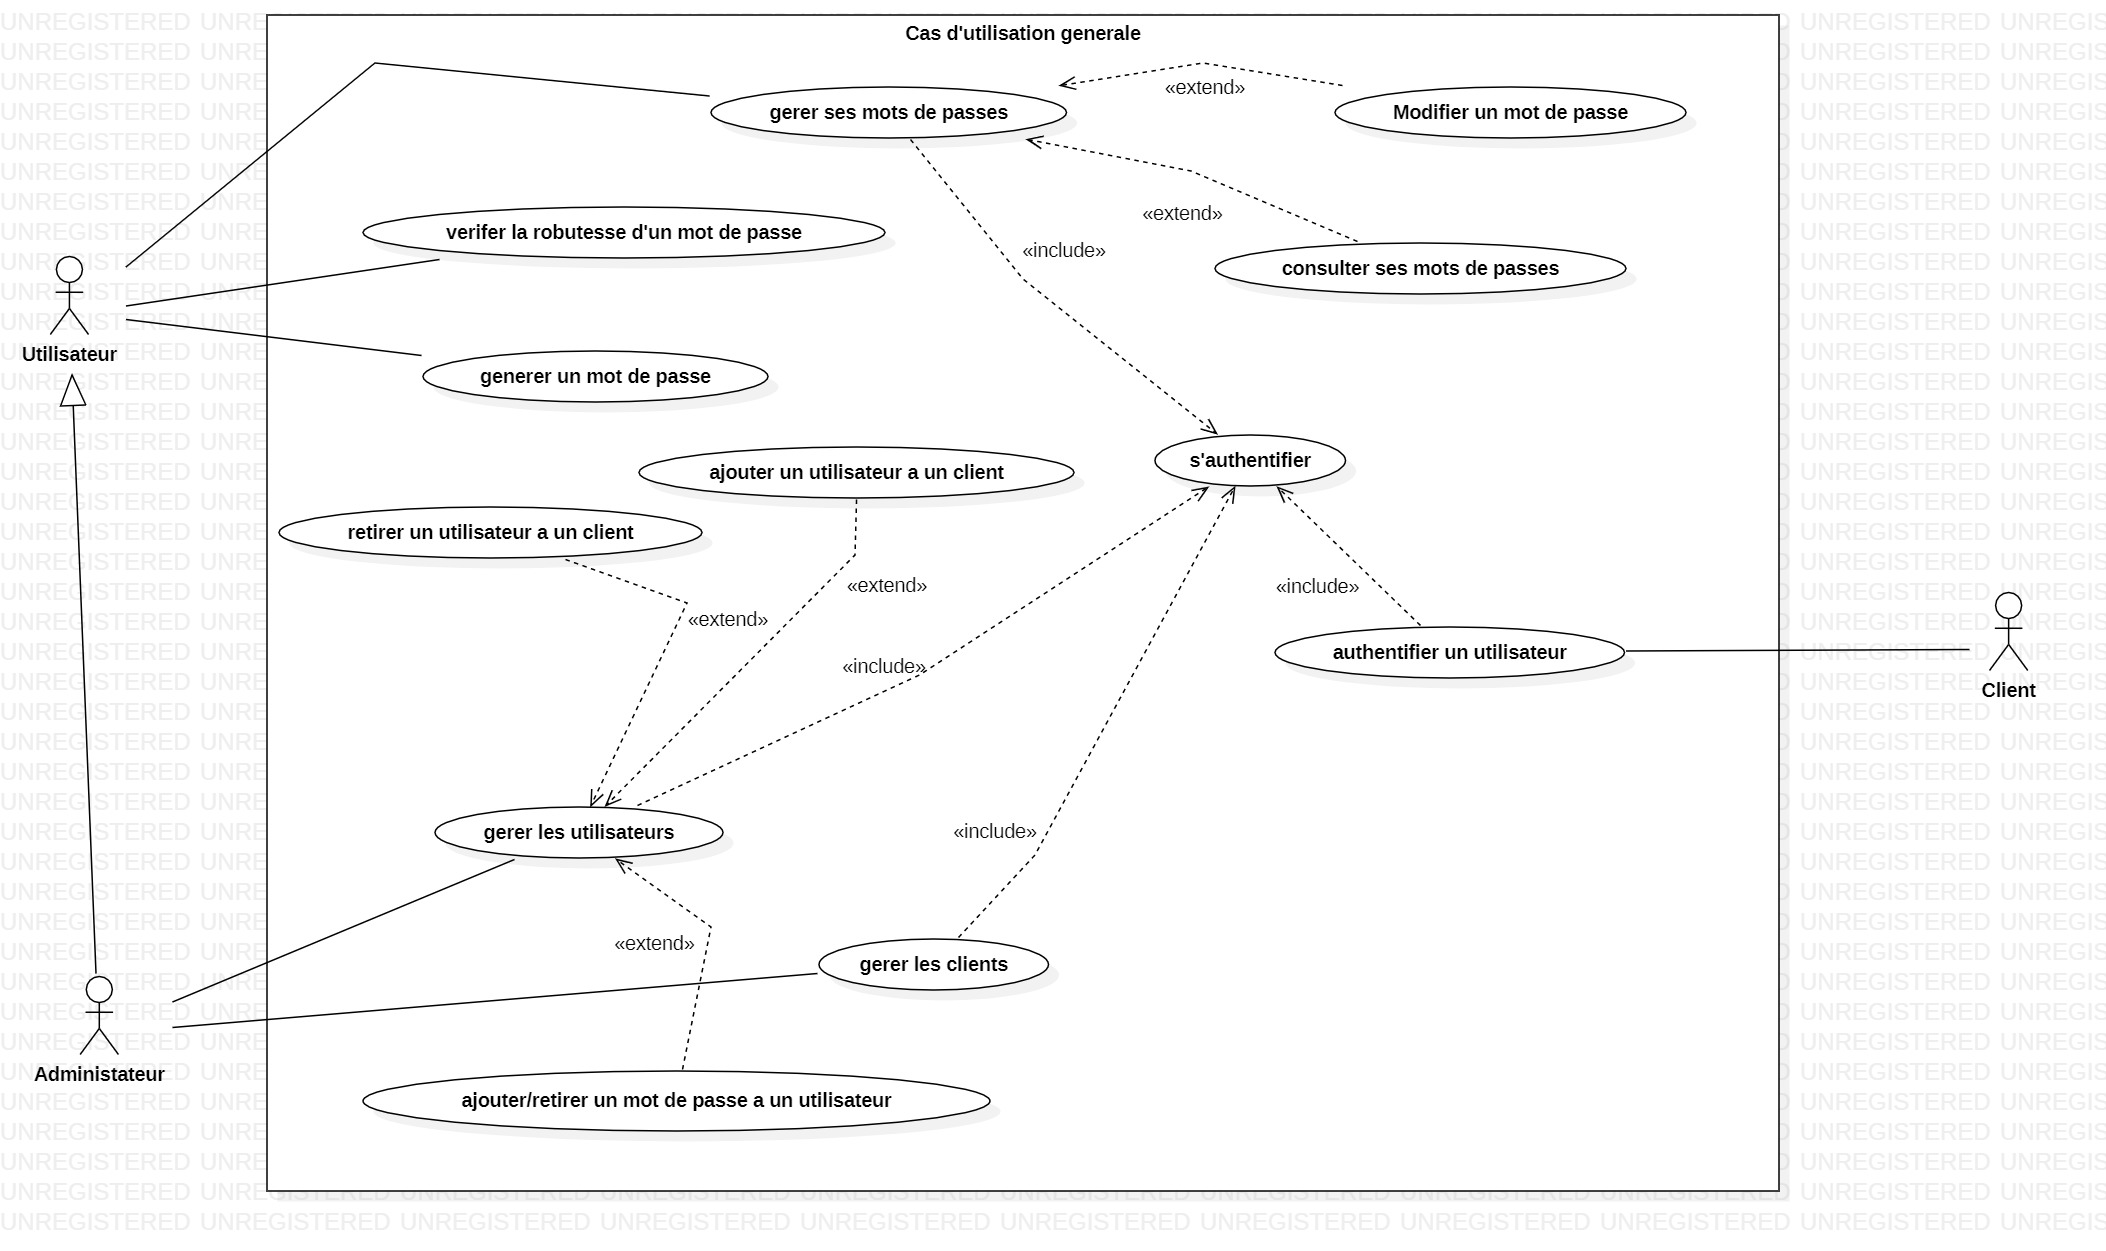
\includegraphics[width=\linewidth]{img/jpg/safeprivacing-cas0.jpg}
 \caption{Cas d'utilisation général}
 \label{fig:diagram1}
 \end{figure}
 \end{center}
 Ici, de manière générale l'administrateur gère les utilisateurs ( les structures et/ou entreprises) qui s'approprient. Autrement dit, lorsque ceux-ci viennent à lui, il les enregistres tout en les communiquant des ID. A son tour, le consumer va mettre à disposition de ses clients un service intégrant . Toutefois, il faut noter que c'est le l'utilisateur qui crée un donne l'accès aux clients.

 \section{Diagramme de séquence}
 
 Le diagramme de séquence est un enchainement précis et ordonnée d'opérations en vue de la réalisation d'un cas d'utilisation ou une fonctionnalité du système.
 \subsection{Authentification}
Dans la figure l'utilisateur rentre ses identifiants et a accès au site et est retourner sur la page d'accueil en cas de succès et reste sur la même page en cas d'erreur. 
\begin{center}
 \begin{figure}[H]
 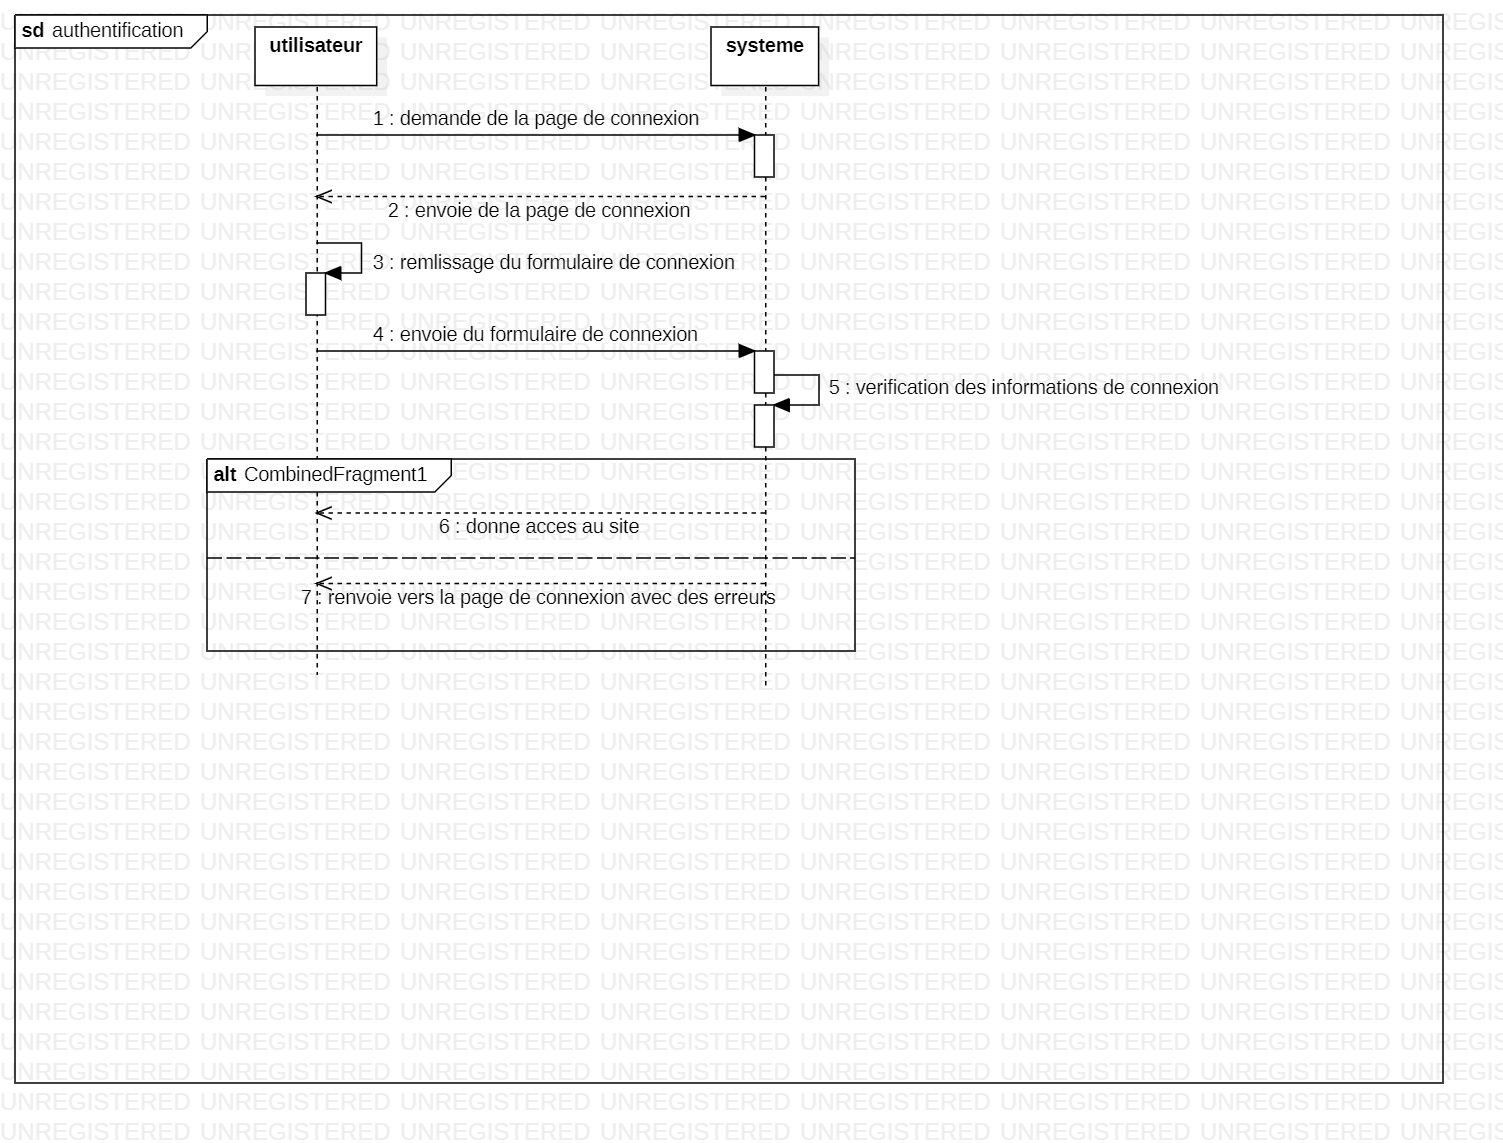
\includegraphics[width=\linewidth]{img/jpg/safeprivacing2.jpg}
 \caption{Authentification}
 \label{fig:diagram2}
 \end{figure}
 \end{center}
 
 \newpage
 \subsection{Gérer les utilisateurs}
 \begin{enumerate}
 \item Création d'un utilisateur \\ 
 
 Dans la figure \ref{fig:diagram3}, une fois l'administrateur est authentifier il a accès à la page d'ajout d'un nouveau utilisateur, il rempli le formulaire avec les informations de l'utilisateur et renvoi au système. Le système ajoute l'utilisateur et renvoi une réponse . 
 \begin{center}
 \begin{figure}[H]
 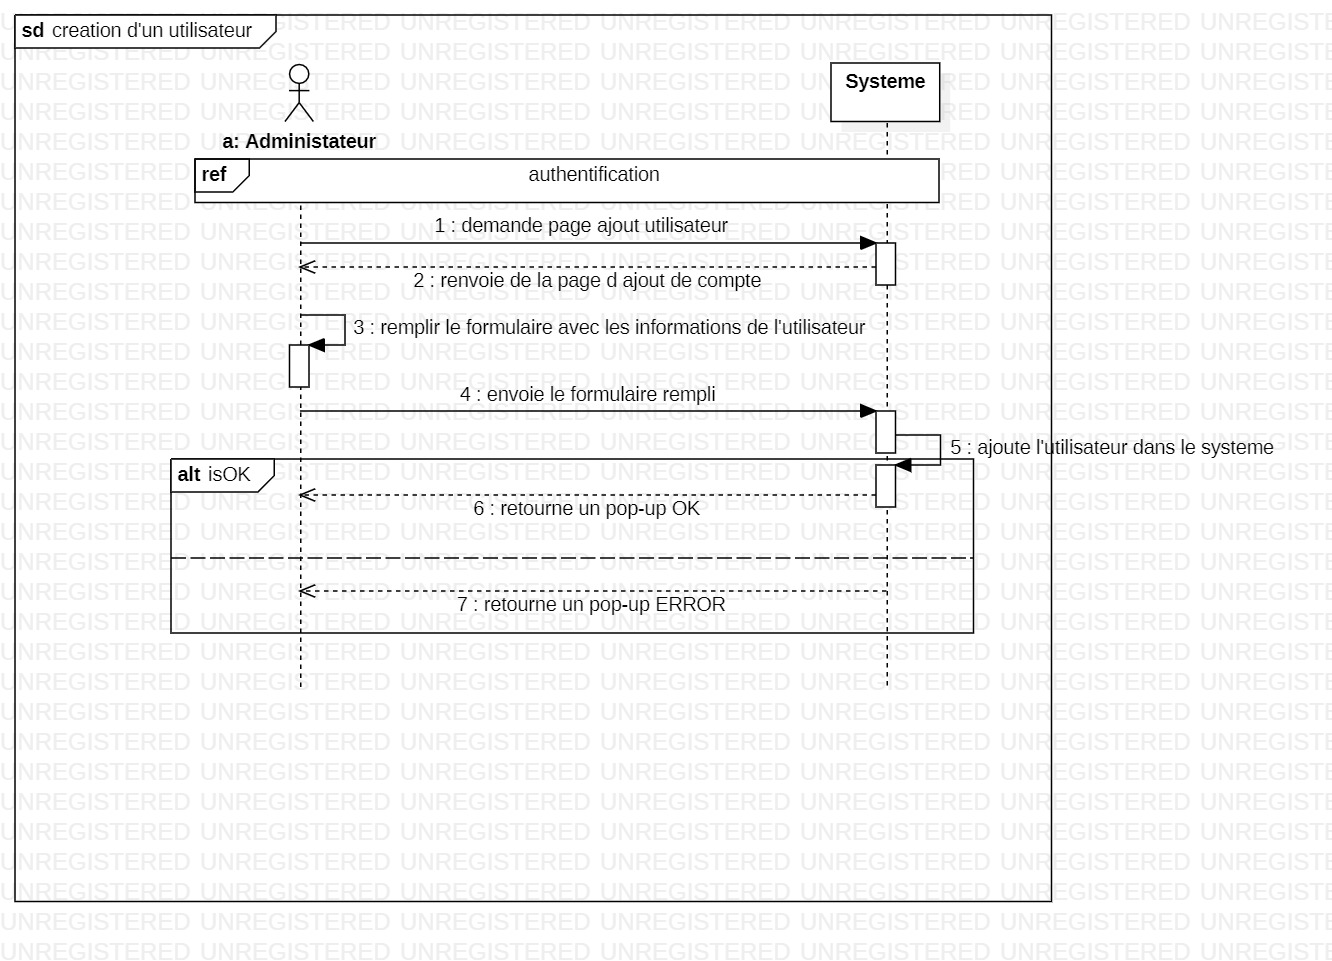
\includegraphics[width=\linewidth]{img/jpg/safeprivacing1.jpg}
 \caption{Création d'un utilisateur}
 \label{fig:diagram3}
 \end{figure}
 \end{center}
\newpage
 \item Suppression d'un utilisateur \\
 
\begin{center}
 \begin{figure}[H]
 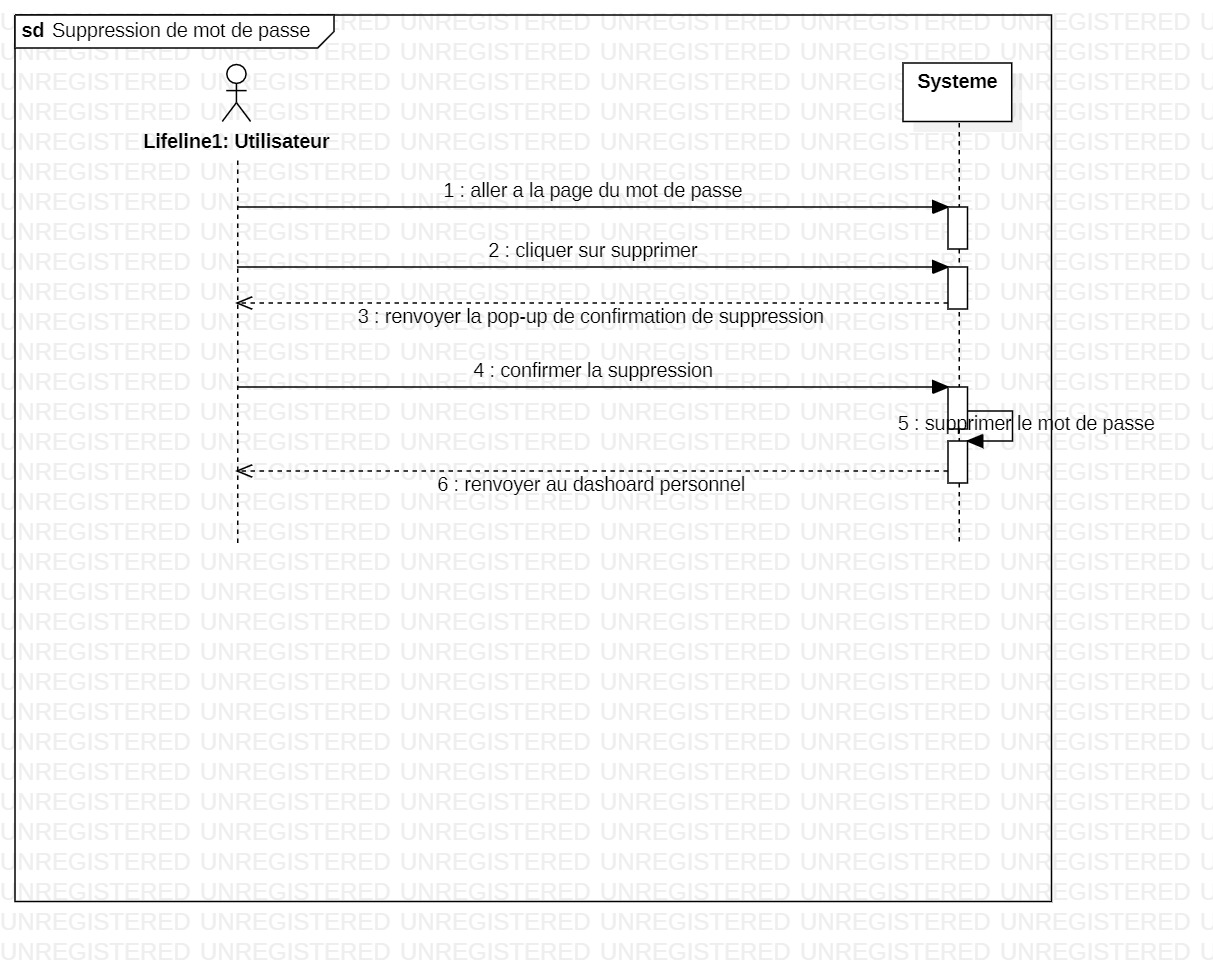
\includegraphics[width=\linewidth]{img/jpg/safeprivacing-suppression5.jpg}
 \caption{Suppression de mot de passe}
 \label{fig:diagram4}
 \end{figure}
 \end{center}
 \newpage
\item Suppression de mot de passe

\begin{center}
 \begin{figure}[H]
 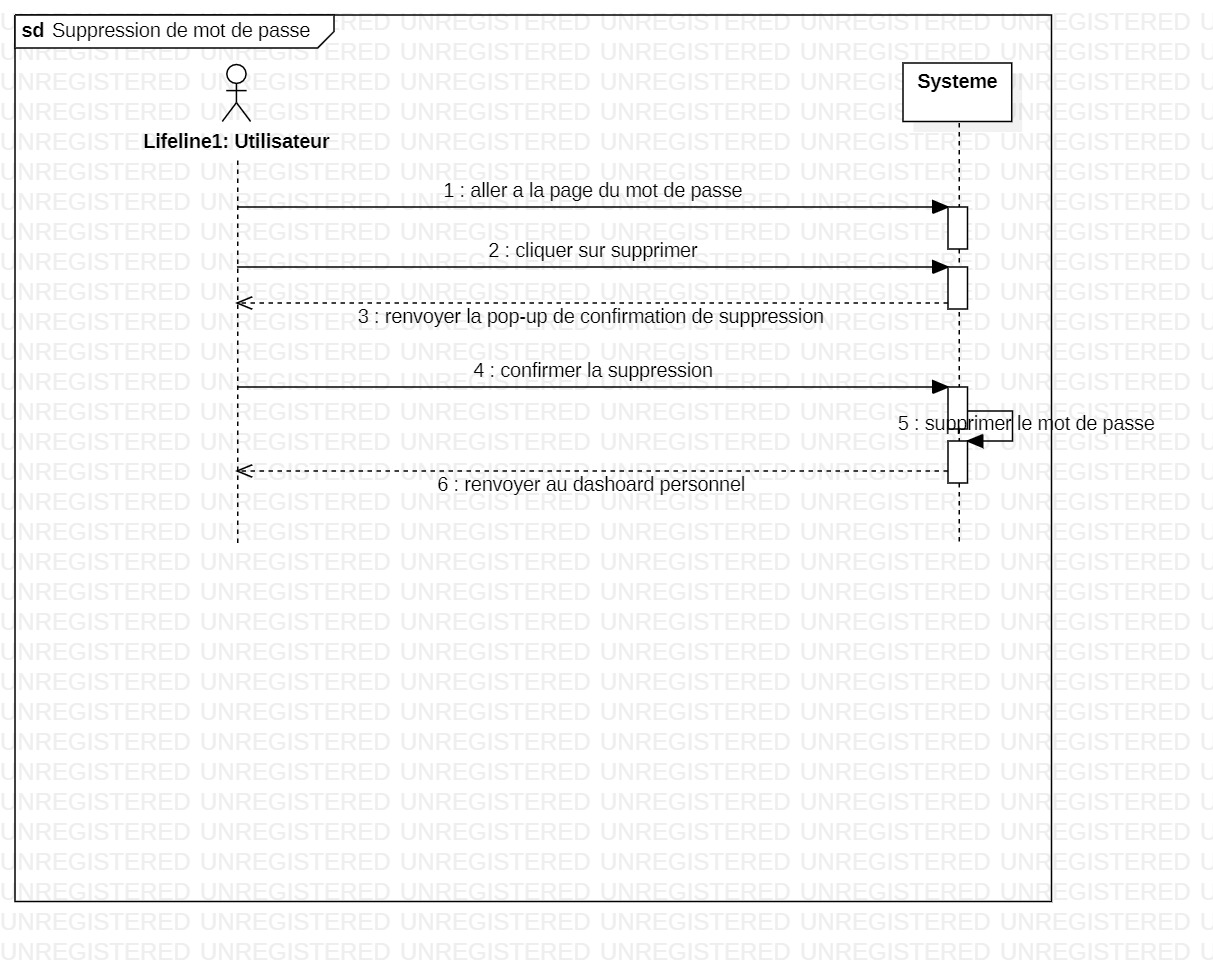
\includegraphics[width=\linewidth]{img/jpg/safeprivacing-suppression5.jpg}
 \caption{Suppression de mot de passe}
 \label{fig:diagram4}
 \end{figure}
 \end{center}
 \newpage
\item Modification de mot de passe
 
\begin{center}
 \begin{figure}[H]
 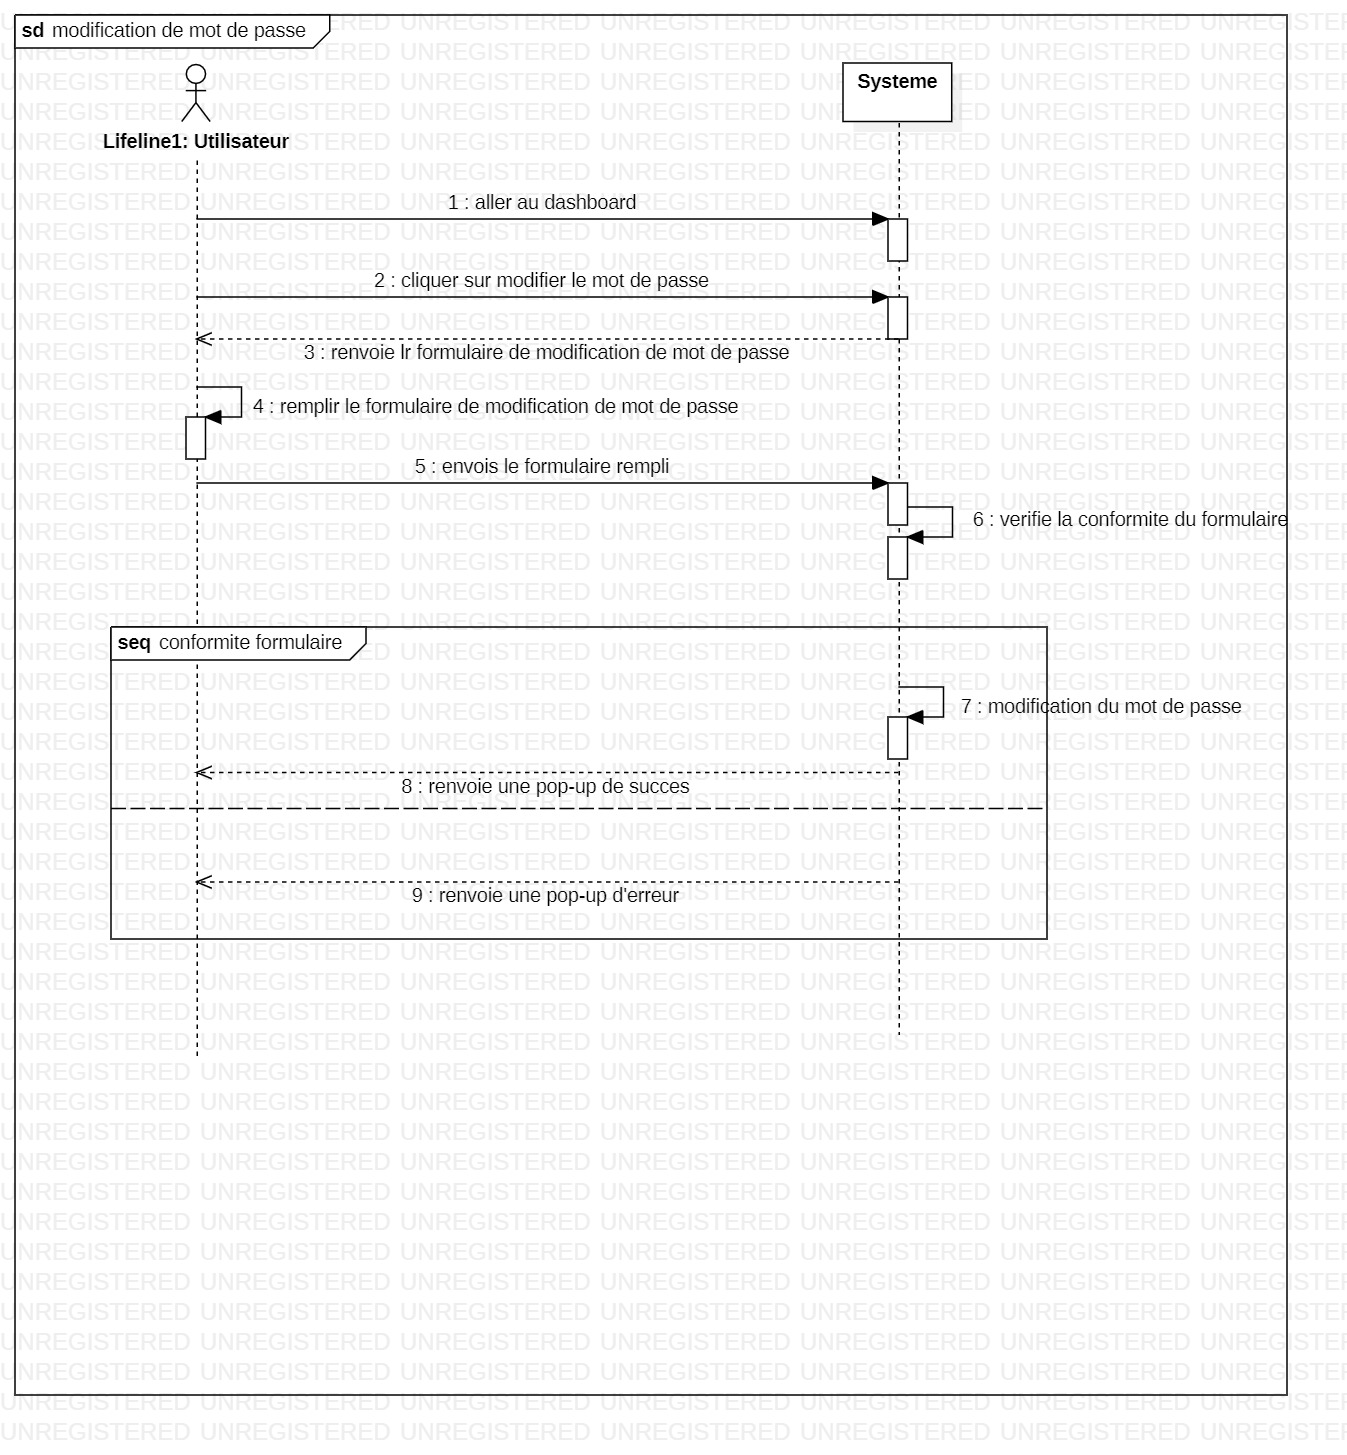
\includegraphics[width=\linewidth]{img/jpg/safeprivacing-modif4.jpg}
 \caption{Modification de mot de passe}
 \label{fig:diagram5}
 \end{figure}
 \end{center}
 
 \end{enumerate}
 \newpage
 \section{Diagramme de Classe}
 
 C'est un diagramme qui fait partie de la partie statique d'UML car il fait abstraction des aspects temporels et dynamiques. Il permet de décrire clairement la structure d'un système en fournissant une représentation abstraite des objets du système qui vont interagir pour réaliser les cas d'utilisations.


 \begin{center}
 \begin{figure}[H]
 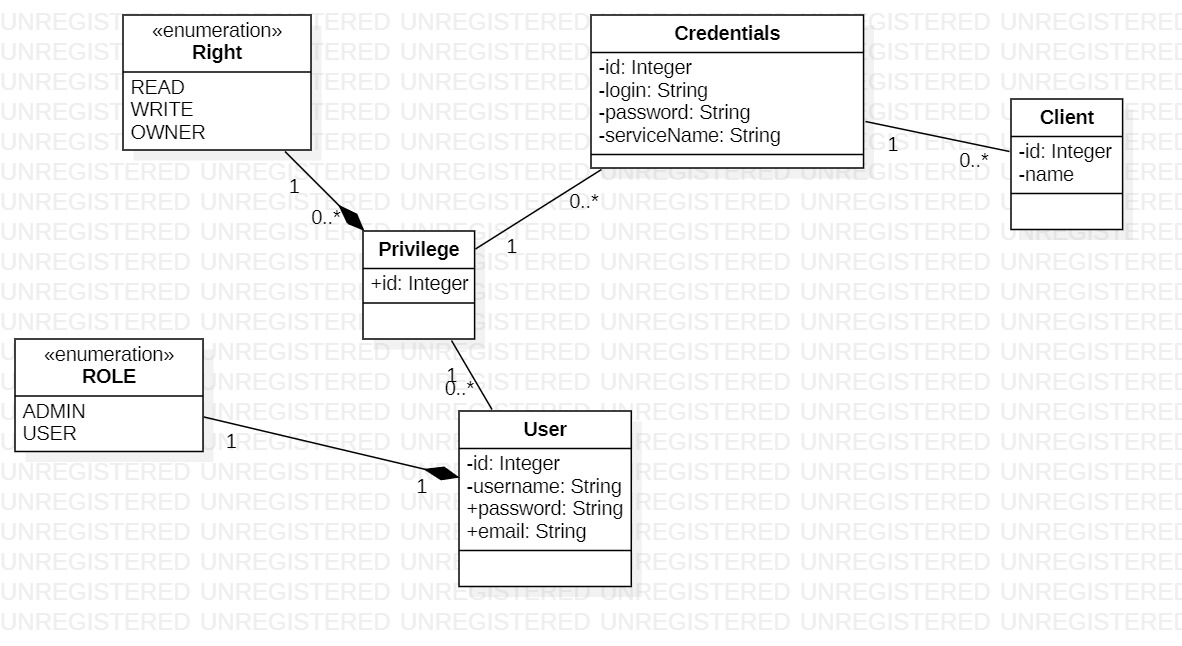
\includegraphics[width=\linewidth]{img/jpg/safeprivacing-diagramme-classe4.jpg}
 \caption{Diagramme de classe}
 \label{fig:diagram6}
 \end{figure}
 \end{center}
 \section{Implémentation}
 
 L'implémentation est l'une des phases phares de ce travail car elle est l'étape à la fin de
laquelle nous obtenons le produit fini de notre projet. Nous présenterons dans un premier temps
les outils backend, puis frontend, les outils globaux et enfin les matériels utilisés.

\subsection{Outils Backend}

 \textbf{Spring Boot} \\ 
Spring Boot peut être défini comme un framework open source basé sur JAVA qui est utilisé pour créer un microservice développé par Pivotal Team, Spring Boot est très applicable pour construire une production prête et une application Spring inégalée.
 \textbf{Java} \\ 
 Java est un langage de programmation orienté objet créé par James Gosling et Patrick Naughton, employés de Sun Microsystems, avec le soutien de Bill Joy (cofondateur de Sun Microsystems en 1982), présenté officiellement le 23 mai 1995 au .SunWorld.
 \textbf{Visual studio code} \\ 
  C'est un éditeur de code extensible développé par Microsoft pour Windows, Linux et
macOS. Les fontionnalités incluent la prise en charge du débogage, la mise en évidence de
la syntaxe, la refactorisation du code et Git intégré.
 
\subsection{Outils Frontend} 

   \textbf{HTML 5} \\ 
   C'est le format de données conçu pour représenter les pages web. C'est un langage de
balisage permettant d'écrire de l'hypertexte
 \textbf{CSS 3} \\ 
   Les feuilles de style en cascade, généralement appelées CSS de l'anglais Cascading Style
Sheets, forment un langage informatique qui décrit la présentation des documents HTML
et XML. Les standards définissant CSS sont publiés par le World Wide Web Consortium
(W3C). Introduit au milieu des années 1990, CSS devient couramment utilisé dans la
conception de sites web et bien pris en charge par les navigateurs web dans les années
2000.
   \textbf{Javascript}\\  
   \textbf{Timelift} \\ 
\subsection{Outils globaux} 
   \textbf{Git} \\ 
Git est un logiciel de gestion de versions décentralisé. C'est un logiciel libre créé par
Linus Torvalds, auteur du noyau Linux, et distribué selon les termes de la licence publique
générale GNU version 2. Cet outil nous a permis de faire des commit pour garder plusieurs
versions de l'API afin de rentrer en arrière dans une situation critique.
   \textbf{StarUML}\\ 
StarUML est un outil de génie logiciel dédié à la modélisation UML et édité par la société
coréenne MKLabs. Il est multi-plateforme et fonctionne sous Windows, Linux et MacOS.

Dans ce chapitre, nous avons présenté la conception, la modélisation ainsi que l'implémentation de notre système. Dans le chapitre suivant, nous exposerons les résultats obtenus
ainsi que quelques commentaires.
\section{Conclusion} 
\chapter{RÉSULTATS ET COMMENTAIRES}

\section{Côté Administrateur} 
\section{Côté Utilisateur}
\section{Conclusion}
Dans ce chapitre, il était question pour nous de montrer les résultats de l'implémentation
de notre application. Nous constatons avec satisfaction que les modules phares qui ont été
implémentés fonctionnent correctement. Il convient donc dans la suite de conclure notre travail
et de donner quelques perspectives pour l'amélioration de notre travail.
\chapter*{CONCLUSION GÉNÉRALE ET PERSPECTIVES}
\addcontentsline {toc}{chapter}{CONCLUSION GÉNÉRALE ET PERSPECTIVES}

En somme, notre travail consistait à la conception et la mise en place d'une application de gestion de mot de passe. Elle permet également aux développeurs de la structure, de
gagner en temps lors de la conception des produits futurs moyennant un espace connexion ne
s'attardant plus de ce fait au développement des modules quasi-similaires. En tenant compte
de notre contexte, ainsi que de la méthodologie, nous avons pu atteindre les objectifs fixés
en réalisant avec succès les fonctionnalités de notre cahier de charges sous réserve de quelques
tâches de l'utilisateur. La prochaine étape du cycle de vie de notre projet consistera à l'intégration
des fonctionnalités du cahier de charges qui sont non achevées, ensuite les tests utilisateurs
serons effectués afin de corriger les bugs. Toutefois notre solution bien que bonne, présente un
certain nombre de limites et peut être améliorée en augmentant les modules du customer, en
permettant une gestion de qualité (connaitre le nombre d'utilisateurs, la fréquence d'utilisation,
etc).

\chapter*{BIBLIOGRAPHIE}
\addcontentsline {toc}{chapter}{BIBLIOGRAPHIE}
\bibliographystyle{plain}
\bibliography{rapport}
\end{document}